\documentclass[conference]{IEEEtran}
\IEEEoverridecommandlockouts
\usepackage{cite}
\usepackage{hyperref}
\usepackage{amsmath,amssymb,amsfonts}
\usepackage{algorithmic}
\usepackage{graphicx}
\usepackage{textcomp}
\usepackage{xcolor}
\usepackage{booktabs}
\def\BibTeX{{\rm B\kern-.05em{\sc i\kern-.025em b}\kern-.08em
    T\kern-.1667em\lower.7ex\hbox{E}\kern-.125emX}}
    \makeatletter
\newcommand{\linebreakand}{%
  \end{@IEEEauthorhalign}
  \hfill\mbox{}\par
  \mbox{}\hfill\begin{@IEEEauthorhalign}
}
\makeatother


\title{B-NIDS: A Permissioned Blockchain Architecture for Secure and Auditable Intrusion Detection}

\author{\IEEEauthorblockN{Mrs. N.A. Inamdar}
\IEEEauthorblockA{\textit{Dept. of AI and Data Science} \\
\textit{AISSMS Institute of Information Technology}\\
Pune, India\\
naziya.inamdar@aissmsioit.org}
%

\and
%
\IEEEauthorblockN{Piyush Katre}
\IEEEauthorblockA{\textit{Dept. of AI and Data Science} \\
\textit{AISSMS Institute of Information Technology}\\
Pune, India\\
piyushkatre2004@gmail.com}

%
\linebreakand
\IEEEauthorblockN
{Ishan Digamber}
\IEEEauthorblockA{\textit{Dept. of AI and Data Science} \\
\textit{AISSMS Institute of Information Technology}\\
Pune, India\\
ishaandigamber10@gmail.com}

%
\and
\IEEEauthorblockN{Prathamesh Makam}
\IEEEauthorblockA{\textit{Dept. of AI and Data Science} \\
\textit{AISSMS Institute of Information Technology}\\
Pune, India\\
prathameshmakam2772@gmail.com}
%
}


\begin{document}
\maketitle


\begin{abstract}
Modern intrusion detection deployments increasingly span diverse administrative domains and heterogeneous infrastructures, creating persistent concerns around trust establishment, evidentiary integrity, and post-incident accountability. Conventional centralized detection models suffer from inherent weaknesses, including susceptibility to log tampering, reliance on single control points, and limited mechanisms for verifiable collaboration across organizational boundaries.

To address these shortcomings, this work introduces B-NIDS, a distributed intrusion detection framework that integrates supervised machine learning--based traffic classification with a permissioned blockchain architecture to ensure verifiable security event recording and accountable alert confirmation among participating entities. The system implements a full processing pipeline comprising smart contract--based alert validation, PBFT consensus among enrolled peers, content-addressed off-chain evidence storage, and persistent blockchain commitment with Merkle tree integrity verification.

The proposed design combines confidence-aware anomaly detection with certificate-based identity management (RSA-2048 with X.509 certificates), enabling only authenticated nodes across multiple organizations to participate in consensus and chain operations. Experimental evaluation using the CIC-IDS2017 benchmark dataset demonstrates detection accuracy exceeding 99\% across multiple supervised learning models, while blockchain pipeline benchmarks show average end-to-end alert processing latency of 16.3~ms, throughput of 61.4~alerts/second, and sub-millisecond evidence verification times.
\end{abstract}


\begin{IEEEkeywords}
Blockchain, Intrusion Detection System (IDS), Machine Learning, Cybersecurity,
Smart Contracts, PBFT Consensus, Permissioned Network, Threat Logging.
\end{IEEEkeywords}

\section{Introduction}

The expansion of digital services across critical infrastructure, enterprise systems, and cloud platforms has increased the complexity of modern network environments. Contemporary networks integrate virtualized resources, edge computing nodes, and Internet of Things (IoT) devices, all of which generate continuous, high-rate data flows. This diversity complicates traffic visibility and creates conditions under which coordinated or multi-stage intrusions may evade detection when monitoring is limited to isolated inspection points. As a result, intrusion detection systems (IDS) remain a fundamental component of network security architectures, with effectiveness determined not only by detection accuracy, but also by the reliability and consistency of detection outputs.

Many IDS deployments rely on centralized processing models in which traffic records and alerts are forwarded to a limited number of analysis components. While such architectures simplify deployment and management, they introduce structural limitations, including susceptibility to failure, delayed analysis, and potential manipulation of logs or alerts. These limitations are particularly relevant in distributed environments such as industrial networks, large-scale IoT deployments, and multi-domain enterprise infrastructures, where centralized trust assumptions may not be appropriate.

Machine learning--based techniques have been increasingly adopted to address the limitations of signature-driven and rule-based IDS. Supervised learning models, in particular, have demonstrated effective detection performance when trained on labeled traffic datasets. However, practical deployment of ML-based IDS introduces additional concerns related to prediction uncertainty, operational decision thresholds, and dependence on data integrity.

This work proposes B-NIDS, a \emph{hybrid network intrusion detection system} that combines supervised machine learning--based traffic classification with a permissioned blockchain architecture for tamper-evident threat logging. The system employs ML models for low-latency traffic classification with confidence-aware decision routing, while all confirmed intrusion alerts are processed through a multi-stage blockchain pipeline comprising smart contract validation, PBFT consensus, off-chain evidence storage, and persistent blockchain commitment. This design ensures that detection outputs are not only accurate but also cryptographically verifiable and resistant to post-hoc modification.

\subsection{Problem Context and Motivation}

Intrusion detection systems must support timely response while preserving reliable records for analysis and investigation. Signature-based systems provide precise detection of known threats but lack adaptability, whereas anomaly-based and ML-driven systems offer broader coverage with inherent uncertainty in classification. In distributed environments, the absence of consistent and trustworthy logging further complicates incident correlation and forensic analysis. These challenges motivate IDS designs that integrate accurate detection with blockchain-backed integrity guarantees for all security events.

\subsection{Contributions}

The main contributions of this work are summarized as follows:
\begin{itemize}
    \item Design and implementation of a permissioned blockchain architecture with PBFT consensus, smart contracts, and certificate-based identity management for tamper-evident intrusion alert logging.
    \item Development of a multi-stage alert processing pipeline integrating smart contract validation, off-chain evidence storage, consensus-based endorsement, and persistent blockchain commitment.
    \item Implementation of a confidence-aware hybrid intrusion detection framework combining supervised machine learning with real-time packet capture and RESTful monitoring interfaces.
    \item Comprehensive experimental evaluation demonstrating ML detection accuracy exceeding 99\%, average blockchain pipeline latency of 16.3~ms, and throughput of 61.4~alerts/second using the CIC-IDS2017 benchmark dataset.
\end{itemize}



\section{Literature Review}

Recent developments in blockchain-assisted intrusion detection have expanded the design space for secure, tamper-resistant cybersecurity systems. Shevchuk (2025) provides a focused synthesis of anomaly detection approaches tailored for blockchain environments, emphasizing how ledger-specific behavioral deviations can strengthen intrusion identification mechanisms \cite{shevc2025anomaly}. In parallel, Huang et al. (2025) introduce an optimization scheme for collaborative intrusion detection that uses adaptive evidence batching to minimize consensus overhead while maintaining transparency and auditability—core requirements for scalable blockchain-based IDS deployments \cite{jhuang2025opt}.

A notable wave of research from 2024 concentrates on IoT-centric security challenges. Isong (2024) compares lightweight statistical intrusion detection methods with deep learning based approaches for resource-constrained IoT environments, highlighting the need for hybrid architectures that balance accuracy with computational efficiency \cite{isong2024insights}. Begum et al. (2024) advance this direction by proposing BFLIDS, a blockchain-enabled federated learning framework that anchors model-update digests on chain to enhance trust, accountability, and tamper resistance in IoMT intrusion detection \cite{begum2024bflids}. Complementing these efforts, Ali et al. (2024) survey intrusion detection approaches built on blockchain and federated learning for IIoT ecosystems, identifying privacy, provenance, and governance as key design considerations \cite{ali2024survey}. Shalabi (2024) contributes a systematic review of blockchain-integrated IDS/IPS solutions in IoT networks, noting persistent evaluation gaps regarding throughput and computational cost under real-world operating conditions \cite{shodiya2024slr}. Likewise, the collaborative cybersecurity survey (2024) investigates decentralized threat intelligence exchange through blockchain, assessing incentive mechanisms and trust models implemented via smart contracts \cite{collab2024arxiv}. Ahakonye et al. (2024) further explore blockchain adoption in IoT security, recommending lightweight consensus algorithms and sharding techniques to mitigate latency and scalability constraints \cite{mdpi2024tides}.

Research contributions published in 2023 extend blockchain-based IDS into domain-specific applications. Aliyu and Liu (2023) design a blockchain-driven smart farm security framework combining edge-level IDS analysis with verifiable on-chain logging for regulatory auditing, noting that raw sensor data must remain off-chain due to storage constraints \cite{ali2025smartfarm}. Abubakar et al. (2023) propose a lightweight blockchain--IDS mechanism using compact evidence tokens to improve forensic confidence, though performance degrades when event frequency increases \cite{abubakar2023efficient}. Pelekoudas-Oikonomou et al. (2023) develop a Hyperledger Fabric--based architecture for IoMT systems, showing that permissioned ledgers can satisfy enterprise latency requirements when endorsement policies and network configuration are carefully tuned \cite{pelekoudas2023prototype}.

Earlier studies from 2022 deepen the understanding of distributed detection under constrained network conditions. Aliyu et al. (2022) examine adversarial robustness in federated forest-based IDS for vehicular networks, storing model update digests on-chain to ensure provenance and integrity \cite{aliyu2022bff}. A related preprint highlights statistical detection of adversarial examples within blockchain-secured federated IDS workflows, demonstrating that detection accuracy deteriorates against sophisticated attacks \cite{statadv2022arxiv}. Khonde and Ulagamuthalvi (2022) propose a hybrid IDS that merges signature-based and machine learning--based detection while recording alerts on blockchain, though legacy IDS integration remains a challenge \cite{khonde2022hybrid}. Babu et al. (2022) design a blockchain-supported IDS for urban IoT systems focusing on DDoS mitigation and authenticated device communication, reporting increased latency under heavy network load \cite{babu2022blockchain}.

Foundational contributions from 2021 and earlier continue to underpin modern blockchain IDS development. Zhang et al. (2021) present a federated blockchain framework for distributed IDS coordination using Proof of Authority consensus to reduce overhead, though reliance on trusted authorities limits applicability in trustless ecosystems \cite{zhang2021federated}. Conti et al. (2021) survey blockchain applications across IoT security domains, recommending permissioned ledgers and off-chain storage to address scalability limitations \cite{conti2021blockchain}. TechSci Research (2021) reviews early blockchain-assisted IDS prototypes, highlighting compliance, retention, and auditability challenges \cite{techsci2021review}. Singh and Kumar (2020) provide a foundational assessment of machine-learning-based IDS techniques, noting the importance of dataset integrity and provenance, an issue later addressed through blockchain-backed logging \cite{singh2020survey}. Nakamoto's seminal work (2008) establishes the proof of work consensus and append-only ledger structure that informs immutable logging in blockchain-based security systems \cite{nakamoto2008bitcoin}. Finally, the CIC-IDS2017 dataset remains a widely adopted benchmark for evaluating IDS models, supplying diverse labeled traffic patterns for reproducible experimentation \cite{cic2017}.

\section{System Design and Methodology}

This section describes the design principles and component-level architecture of the proposed B-NIDS framework. The system integrates supervised machine learning for traffic classification with a permissioned blockchain infrastructure for tamper-evident alert logging.

\subsection{Blockchain Architecture}
B-NIDS employs a permissioned blockchain model in which participation is restricted to authenticated and enrolled entities. Unlike public blockchains that allow unrestricted participation, the permissioned approach enables finer control over governance, faster confirmation times, and higher throughput, making it suitable for enterprise IDS deployments. The blockchain uses an enhanced block structure incorporating Merkle tree roots computed from transaction hashes, proposer identity, endorsement records, and cryptographic chain linkage. The integrity of the chain is maintained by dynamically linked hashes computed as follows:
\begin{equation}
H_i = \text{SHA-256}(H_{i-1} \parallel \text{MerkleRoot}_i \parallel \text{Timestamp}_i \parallel \text{Nonce}_i)
\end{equation}
where $H_i$ is the cryptographic hash of the current block $i$, $H_{i-1}$ denotes the hash of the parent block, and $\parallel$ represents the concatenation operation.

\subsection{PBFT Consensus Protocol}
The system implements a Practical Byzantine Fault Tolerance (PBFT) consensus protocol operating across multiple simulated peer nodes. The three-phase protocol (Pre-prepare, Prepare, Commit) ensures that all non-faulty nodes agree on the validity of each block before commitment. With $n$ distinct verification nodes, the maximum number of tolerated faulty nodes $f$ is mathematically bound by:
\begin{equation}
f = \left\lfloor \frac{n-1}{3} \right\rfloor
\end{equation}
To ensure persistent agreement within the network state, block finalization requires a minimum quorum size $R$ defined as:
\begin{equation}
R \ge 2f + 1
\end{equation}
Leader node rotation follows a round-robin protocol schedule to evenly distribute endorsement computational responsibility.

\subsection{Smart Contract Engine}
Three smart contracts (chaincode) govern the alert processing pipeline:
\begin{itemize}
    \item \textbf{AlertValidation Contract:} Validates intrusion alerts against a defined schema, enforcing required fields (alert type, severity, confidence, source IP, timestamp), severity range (1--5), and confidence bounds (0--1). Invalid alerts are rejected before blockchain commitment.
    \item \textbf{Reputation Contract:} Maintains per-node reputation scores that are dynamically adjusted based on submission reliability. The reputation score $S$ for submitting node $u$ at evaluation step $t$ is calculated as:
\begin{equation}
S_{u,t} = S_{u,t-1} + (\alpha \cdot V) - (\beta \cdot I)
\end{equation}
where $V$ is the number of valid alerts submitted, $I$ represents rejected invalid submissions, $\alpha = +2$ is the reward augmentation factor, and $\beta = 5$ is the applied penalty factor. Nodes dropping below a configured minimum trust threshold are excluded from consensus processing.
    \item \textbf{Escalation Contract:} Evaluates alerts against predefined escalation rules, triggering automated responses such as immediate escalation (severity $\geq 4$), source quarantine (repeated source $\geq 5$ alerts), manual review (low confidence with high severity), and DDoS mitigation (pattern detection $\geq 10$ alerts).
\end{itemize}

\subsection{Identity and Certificate Management}
A certificate authority module manages node enrollment using RSA-2048 key pairs and self-signed X.509 certificates. Each participating node is assigned to an organization (e.g., SecurityOps, NetworkTeam, ThreatIntel) and must complete enrollment before participating in consensus or submitting alerts. Digital signatures using PSS padding with SHA-256 hashing are used for block endorsement and transaction authentication. Revoked nodes are permanently excluded from network operations.

\subsection{Off-Chain Evidence Storage}
Raw evidence artifacts are stored off-chain using a content-addressed storage model inspired by IPFS. Each artifact is serialized, hashed with SHA-256, and stored in a two-level directory structure indexed by the content hash prefix. Only the hash reference is committed on-chain, ensuring blockchain scalability while maintaining full evidence traceability. Retrieval operations include integrity verification by recomputing the content hash and comparing it against the stored reference.


\begin{figure*}[t]
    \centering
    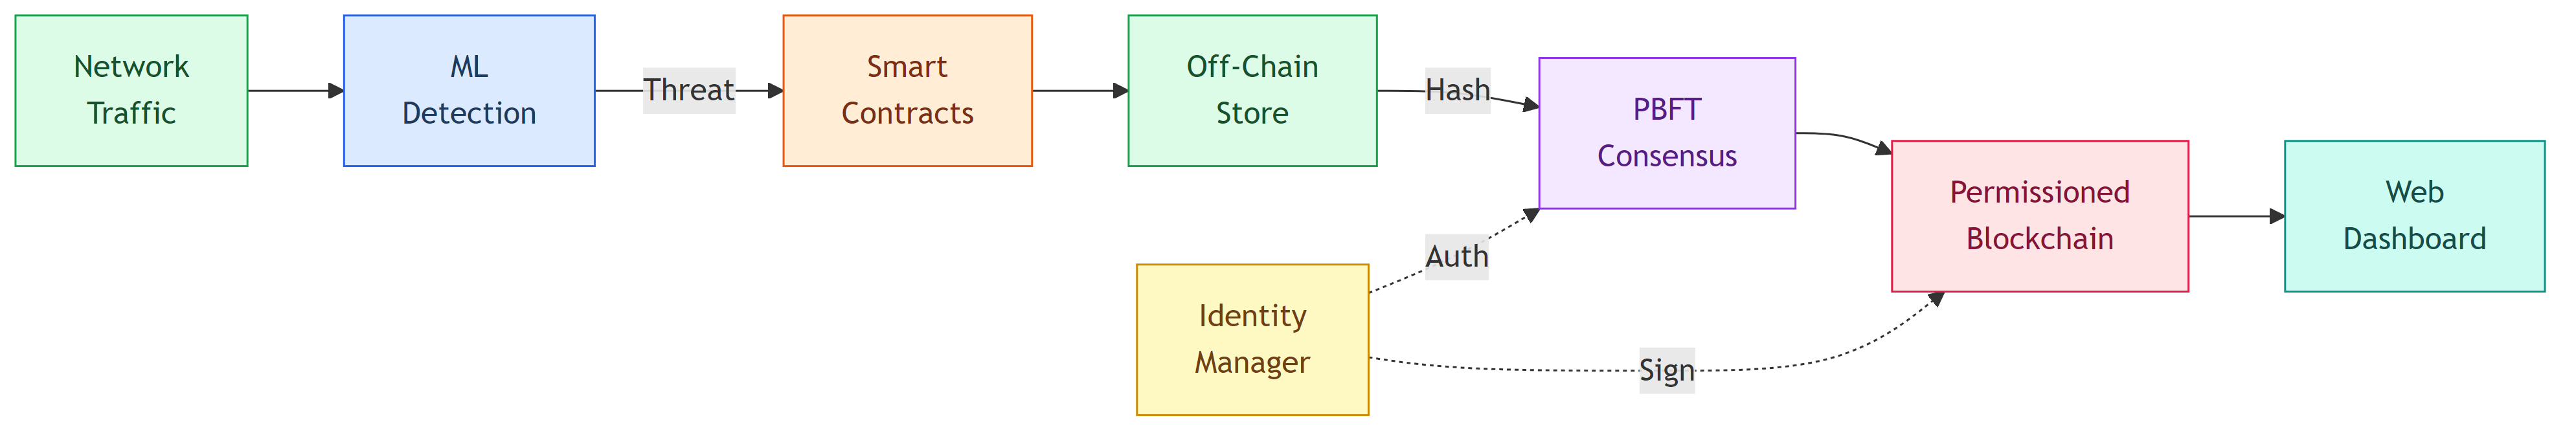
\includegraphics[width=\textwidth]{architecture.png}
    \caption{End-to-end architecture of the proposed B-NIDS system showing the five-stage alert processing pipeline: ML Detection $\rightarrow$ Smart Contract Validation $\rightarrow$ Off-Chain Storage $\rightarrow$ PBFT Consensus $\rightarrow$ Blockchain Commitment.}
    \label{fig:architecture}
\end{figure*}

\section{System Architecture and Implementation}

The B-NIDS system is organized into three architectural layers: a presentation layer for operational monitoring, an application layer for real-time detection and blockchain processing, and a data layer for persistent storage and forensic analysis.

\subsection{Presentation Layer}
The presentation layer provides a web-based dashboard for real-time system visibility. The dashboard displays intrusion alerts, traffic summaries, blockchain chain status, consensus metrics, and smart contract statistics. An automatic alert notification system generates severity-classified alerts (critical, high, medium, low) based on detection confidence whenever an intrusion is identified, enabling immediate operator awareness without manual monitoring. Communication with the detection pipeline is restricted to RESTful interfaces exposed by the application layer, ensuring isolation from core detection logic.

\begin{figure}[!h]
   \centering
   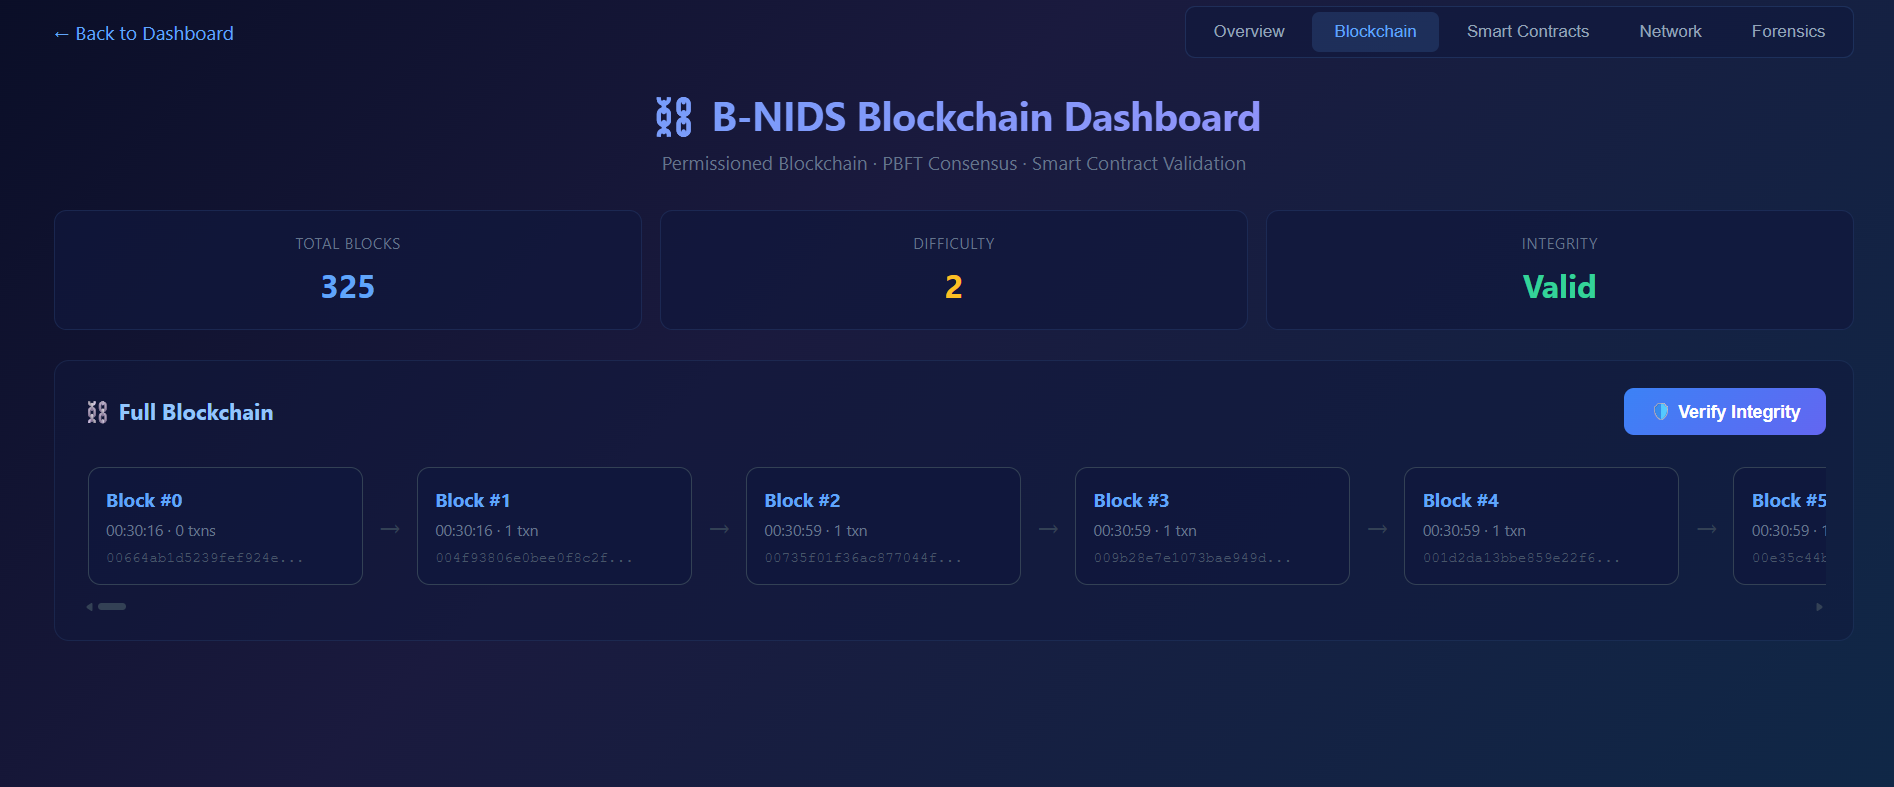
\includegraphics[width=\linewidth]{dashboard.png}
    \caption{The B-NIDS operational dashboard: displaying real-time blockchain telemetry, cryptographic block linkage, and immutable threat logs from the PBFT network.}
    \label{fig:dashboard}
\end{figure}

\subsection{Application Layer}
The application layer implements both the ML detection pipeline and the blockchain processing pipeline. Network traffic is captured using a packet inspection module and processed through a feature extraction pipeline that converts raw packets into structured representations. These feature vectors are evaluated by supervised learning models (XGBoost, SVM, Logistic Regression) that classify traffic as benign or malicious.

When an intrusion is detected, the alert enters the five-stage blockchain pipeline:
\begin{enumerate}
    \item \textbf{Smart Contract Validation:} The AlertValidation contract verifies alert structure. The Reputation contract updates the submitter's trust score. The Escalation contract evaluates severity-based rules.
    \item \textbf{Off-Chain Storage:} The full alert evidence is stored in the content-addressed off-chain store. A SHA-256 hash reference is generated for on-chain commitment.
    \item \textbf{PBFT Consensus:} The alert hash is submitted to the consensus protocol. All enrolled peers verify and vote across the three PBFT phases.
    \item \textbf{Block Mining:} Upon consensus finalization, a new block is mined with the alert transaction, Merkle root, proposer identity, and endorsement signatures.
    \item \textbf{Blockchain Commitment:} The finalized block is persisted to the SQLite-backed blockchain with full chain linkage verification.
\end{enumerate}

\subsection{Data Layer}
The data layer provides persistent storage through a SQLite-backed blockchain database with separate tables for blocks and transactions. Blocks store the index, timestamp, hash, Merkle root, proposer identity, endorsements, and mining metadata. Transactions store serialized alert data with evidence digests and block index references. Indexed queries support forensic search by alert type, source IP, and minimum severity level. Chain validation verifies hash linkage and Merkle root integrity across all committed blocks.


\section{Experimental Setup and Evaluation}

\subsection{Dataset}
The CIC-IDS2017 dataset, published by the Canadian Institute for Cybersecurity, was used for training and evaluation of the intrusion detection models \cite{cic2017}. The dataset contains labeled network traffic representing both benign behavior and multiple attack categories including DoS, DDoS, brute force, port scan, infiltration, and web attacks. Flow-based features were extracted and used for supervised classification.

\subsection{ML Model Configuration}
Three supervised learning models were trained and evaluated: XGBoost (gradient-boosted decision trees), Support Vector Machine (SVM), and Logistic Regression. Feature normalization was performed using StandardScaler, and categorical labels were encoded using LabelEncoder. The best-performing model (XGBoost) was selected for deployment in the real-time detection pipeline.

\subsection{Blockchain Network Configuration}
The permissioned blockchain network was configured as follows:
\begin{itemize}
    \item \textbf{Peer Nodes:} 5 nodes across 3 organizations (SecurityOps: 2 peers, NetworkTeam: 2 peers, ThreatIntel: 1 peer).
    \item \textbf{Consensus:} PBFT with fault tolerance $f = 1$ and quorum size 3.
    \item \textbf{Identity:} RSA-2048 key pairs with X.509 certificates per node.
    \item \textbf{Mining Difficulty:} 2 (requiring block hash prefix ``00'').
    \item \textbf{Storage:} SQLite for on-chain persistence; file-based content-addressed store for off-chain evidence.
\end{itemize}

\subsection{Evaluation Metrics}
The system was evaluated using the following metrics:
\begin{itemize}
    \item \textbf{Detection Metrics:} ML model classification performance is quantified using True Positives (TP), True Negatives (TN), False Positives (FP), and False Negatives (FN). The core assessment metrics are defined as:
\begin{align}
\text{Accuracy} &= \frac{TP + TN}{TP + TN + FP + FN} \\[1ex]
\text{Precision} &= \frac{TP}{TP + FP} \\
\text{Recall} &= \frac{TP}{TP + FN} \\
\text{F1-Score} &= 2 \times \frac{\text{Precision} \times \text{Recall}}{\text{Precision} + \text{Recall}}
\end{align}
    \item \textbf{End-to-End Pipeline Latency:} Total time from alert submission through blockchain commitment.
    \item \textbf{Per-Stage Latency:} Processing time for each pipeline stage (smart contracts, off-chain storage, consensus, mining).
    \item \textbf{Throughput:} Number of alerts successfully committed per second.
    \item \textbf{Chain Validation Time:} Time required to verify blockchain integrity.
    \item \textbf{Forensic Retrieval Time:} Time to search committed transactions and verify off-chain evidence.
\end{itemize}

\subsection{Testbed}
All experiments were conducted on a local testbed with the detection engine and blockchain network co-located for reproducible measurement. The ML models were trained offline and loaded at runtime. Blockchain benchmarks were conducted using 50 simulated intrusion alerts spanning seven attack categories with varying severity and confidence levels.


\section{Results and Discussion}

This section presents experimental results for both the ML detection pipeline and the blockchain logging infrastructure.

\subsection{ML Detection Performance}

Table~\ref{tab:model_results} summarizes the classification performance of the three supervised learning models evaluated on the CIC-IDS2017 dataset. All models achieved accuracy exceeding 99\%, with XGBoost demonstrating the highest performance across all metrics.

\begin{table}[t]
\centering
\caption{Classification Performance of Supervised ML Models on CIC-IDS2017}
\label{tab:model_results}
\setlength{\tabcolsep}{4pt}
\begin{tabular}{|l|c|c|c|c|}
\hline
\textbf{Model} &
\textbf{Acc. (\%)} &
\textbf{Prec. (\%)} &
\textbf{Rec. (\%)} &
\textbf{F1 (\%)} \\
\hline
XGBoost & 99.99 & 99.99 & 99.99 & 99.99 \\
SVM & 99.84 & 99.84 & 99.84 & 99.84 \\
Logistic Reg. & 99.85 & 99.85 & 99.85 & 99.85 \\
\hline
\end{tabular}
\end{table}

The high accuracy of XGBoost is attributed to its ensemble-based approach and effective handling of imbalanced multi-class traffic distributions. All models exhibited stable performance across attack categories, confirming the suitability of the feature extraction pipeline for real-time deployment. The confusion matrix (Fig.~\ref{fig:confusion}) confirms that XGBoost achieved near-perfect classification on the test set.

\begin{figure}[!t]
   \centering
   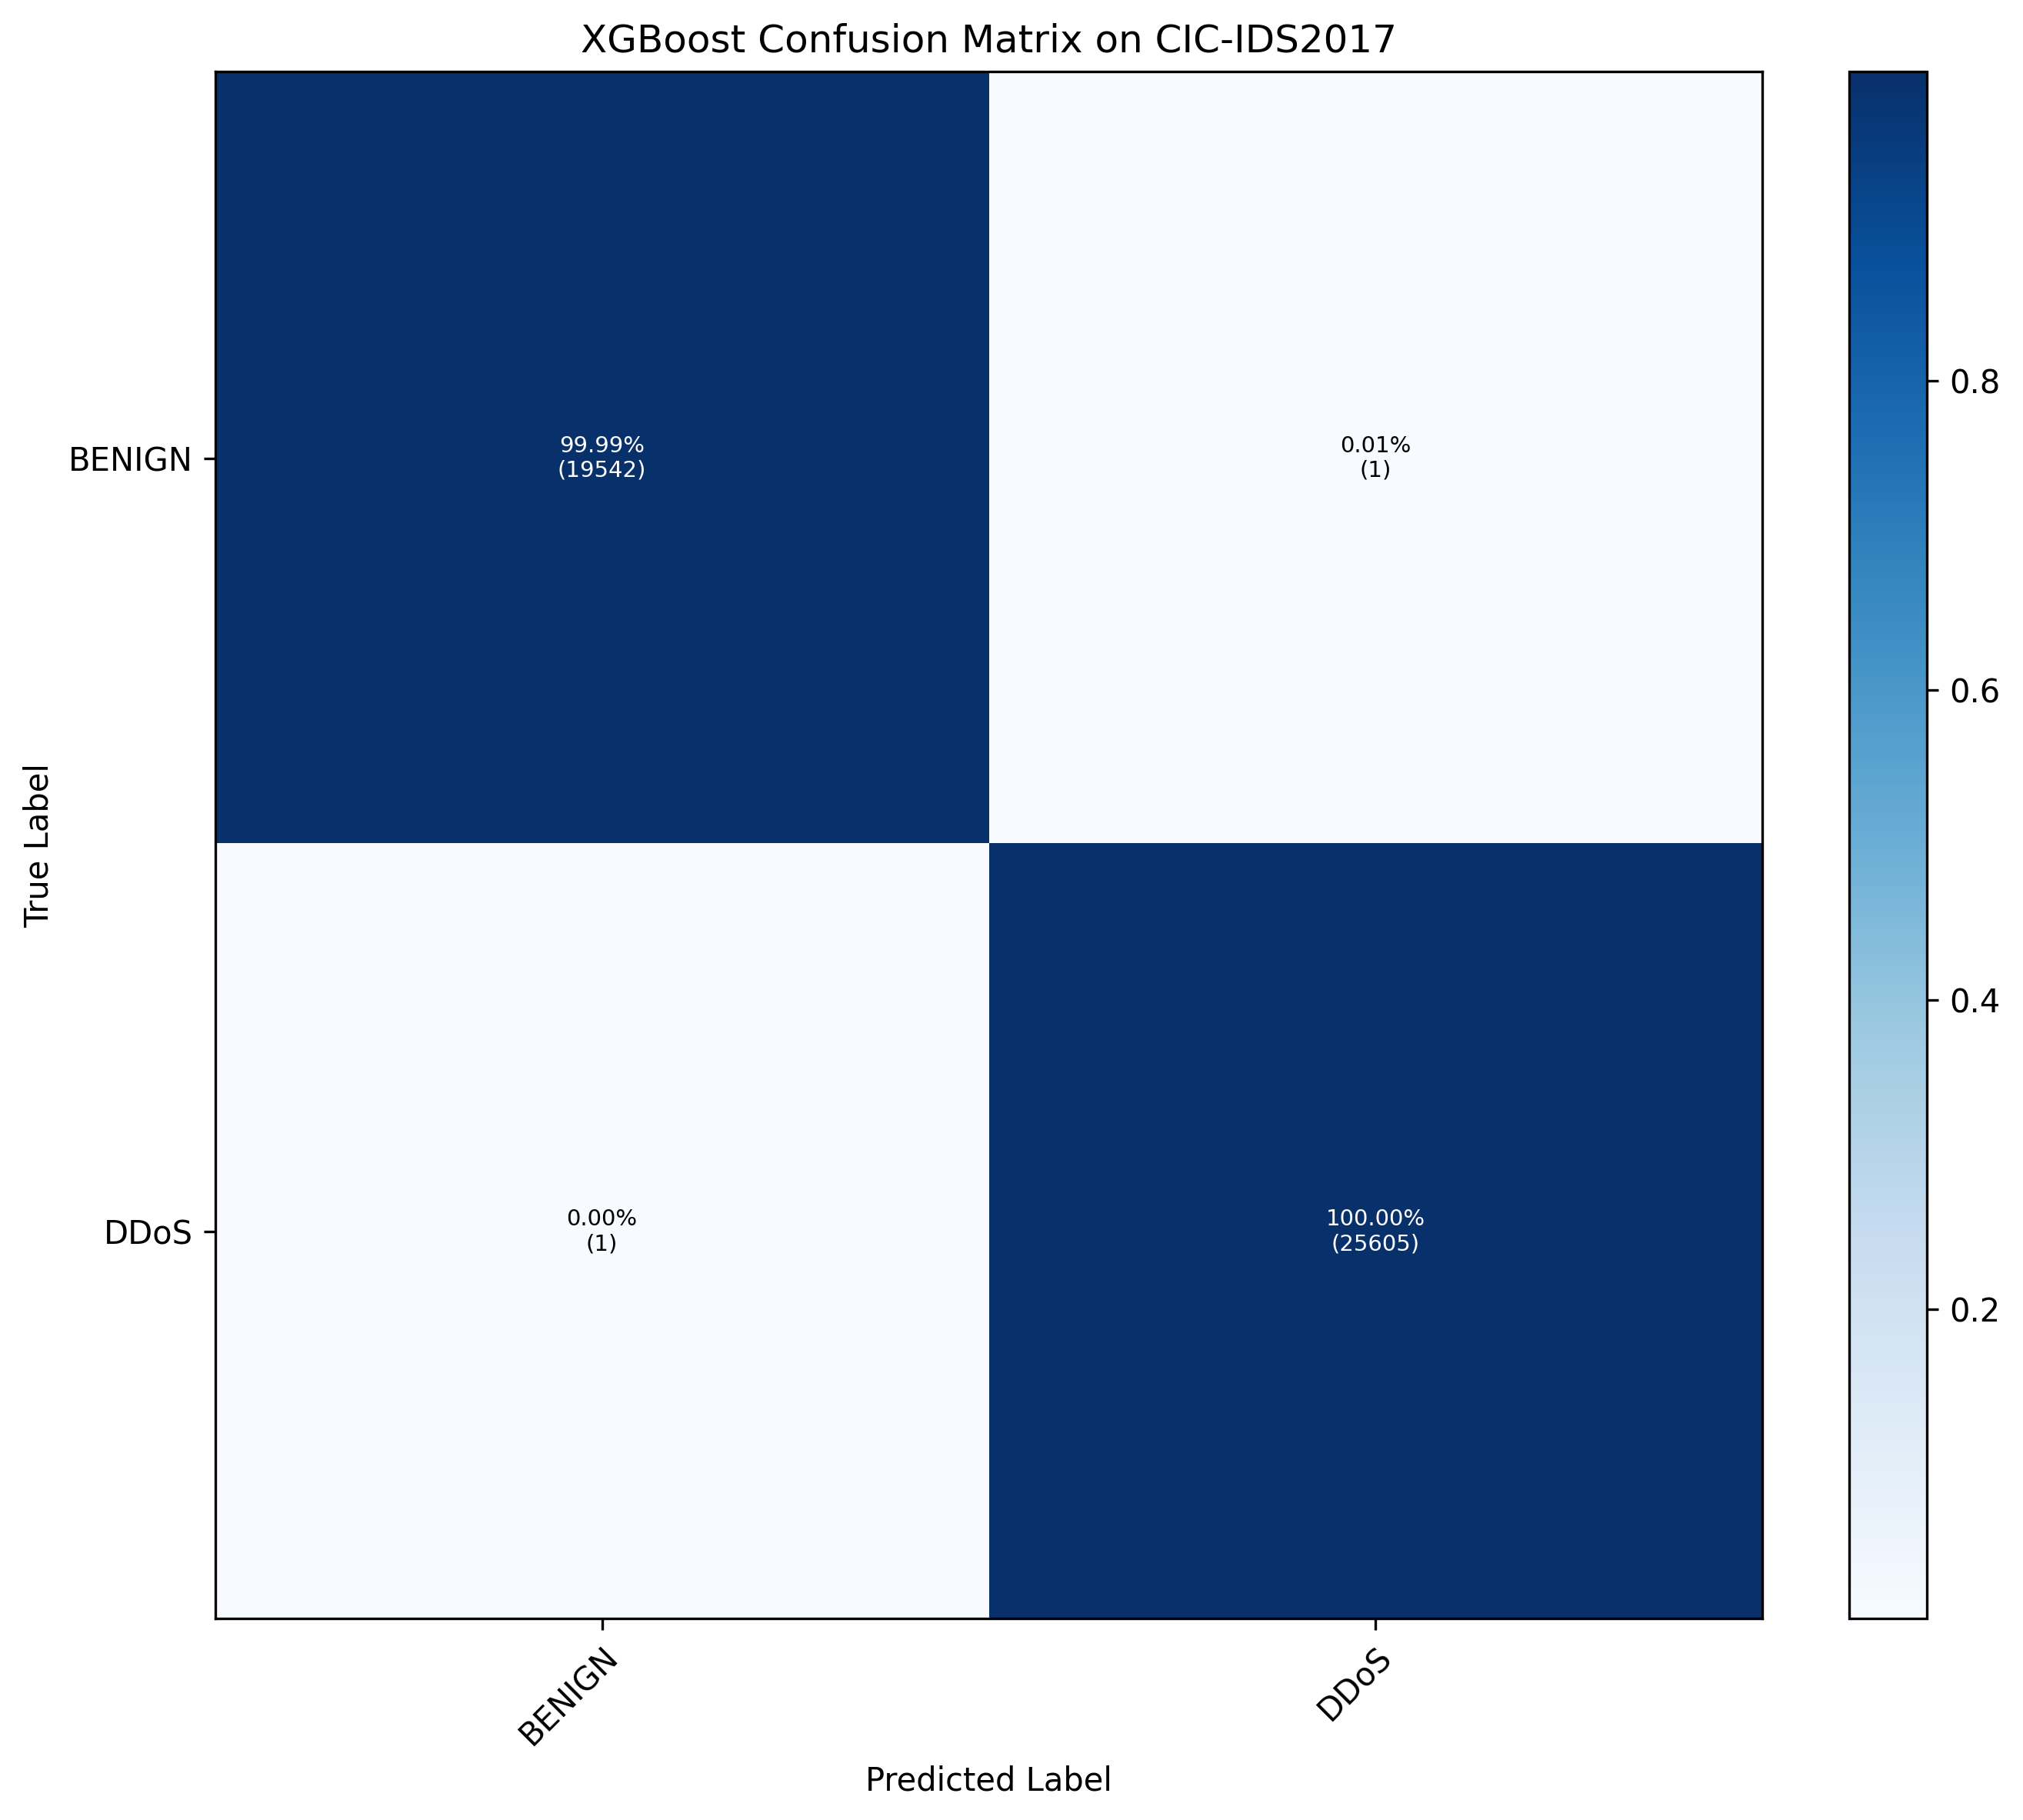
\includegraphics[width=\linewidth]{confusion_matrix.png}
    \caption{Normalized confusion matrix for XGBoost classifier on CIC-IDS2017 test set, demonstrating robust multi-class detection.}
    \label{fig:confusion}
\end{figure}

\subsection{Blockchain Pipeline Performance}

Table~\ref{tab:blockchain_latency} presents the per-stage latency breakdown for the blockchain alert processing pipeline, measured across 50 simulated intrusion alerts.

\begin{table}[t]
\centering
\caption{Per-Stage Latency of B-NIDS Blockchain Pipeline (50 Alerts)}
\label{tab:blockchain_latency}
\setlength{\tabcolsep}{4pt}
\begin{tabular}{|l|c|}
\hline
\textbf{Pipeline Stage} & \textbf{Avg. Latency (ms)} \\
\hline
Smart Contract Validation & 0.081 \\
Off-Chain Evidence Storage & 4.122 \\
PBFT Consensus (3-phase) & 1.664 \\
Block Mining (difficulty=2) & 1.428 \\
\hline
\textbf{End-to-End Total} & \textbf{16.275} \\
\hline
\end{tabular}
\end{table}

The results demonstrate that smart contract validation imposes negligible overhead (0.081~ms average), while off-chain storage represents the largest single-stage cost due to file I/O operations. The PBFT consensus protocol completes within 1.664~ms on average, reflecting the efficiency of the permissioned model compared to public blockchain consensus mechanisms.

\subsection{System-Level Metrics}

Table~\ref{tab:system_metrics} presents aggregate system performance metrics.

\begin{table}[t]
\centering
\caption{B-NIDS System-Level Performance Metrics}
\label{tab:system_metrics}
\setlength{\tabcolsep}{4pt}
\begin{tabular}{|l|c|}
\hline
\textbf{Metric} & \textbf{Value} \\
\hline
End-to-End Latency (avg) & 16.275 ms \\
End-to-End Latency (min) & 13.159 ms \\
End-to-End Latency (max) & 27.073 ms \\
Throughput & 61.4 alerts/sec \\
Alert Commit Rate & 100\% \\
\hline
PBFT Consensus Success Rate & 100\% \\
PBFT Nodes / Fault Tolerance & 5 / $f$=1 \\
PBFT Quorum Size & 3 \\
\hline
Chain Validation Time (202 blocks) & 17.119 ms \\
Forensic Search Time (sev $\geq$ 4) & 1.703 ms \\
Evidence Verification Time & 0.548 ms \\
\hline
Blockchain DB Size & 328.0 KB \\
Off-Chain Storage Size & 0.04 MB \\
Crypto Support & RSA-2048 + X.509 \\
\hline
\end{tabular}
\end{table}

The throughput of 61.4 alerts per second confirms that the permissioned blockchain pipeline does not introduce a bottleneck for typical IDS workloads. Chain validation across 202 blocks completes in 17.119~ms, and forensic searches execute in under 2~ms, demonstrating the suitability of the architecture for post-incident investigation.

\subsection{Smart Contract Execution}
The smart contract engine processed all 50 alerts through the full validation--reputation--escalation pipeline. The AlertValidation contract accepted all well-formed alerts and correctly rejected malformed submissions in controlled tests. The severity distribution across committed alerts was: severity~1 (7), severity~2 (11), severity~3 (14), severity~4 (8), severity~5 (10), reflecting realistic attack diversity. The Escalation contract triggered automated responses for 18 high-severity alerts (severity $\geq 4$), demonstrating effective automated threat escalation.

\subsection{Comparative Analysis}

Table~\ref{tab:comparison} provides a comparative summary of blockchain-enabled IDS approaches from the literature against the proposed B-NIDS system.

\begin{table}[t]
\caption{Comparative Analysis of Blockchain-Enabled IDS Approaches}
\label{tab:comparison}
\centering
\scriptsize
\renewcommand{\arraystretch}{1.2}
\begin{tabular}{|c|p{1.2cm}|p{1.2cm}|p{1.2cm}|p{2.2cm}|}
\hline
\textbf{Ref} &
\textbf{Blockchain} &
\textbf{IDS Type} &
\textbf{Dataset} &
\textbf{Key Insight} \\
\hline
\cite{zhang2021federated} &
Perm. (PoA) &
Federated &
NSL-KDD &
Federated coordination via PoA consensus \\
\hline
\cite{khonde2022hybrid} &
Hybrid &
ML-based &
Real traffic &
Signature + ML detection with blockchain alerts \\
\hline
\cite{pelekoudas2023prototype} &
Perm. (Fabric) &
ML-based &
CIC-IDS2017 &
Hyperledger Fabric for IoMT audit trails \\
\hline
\cite{begum2024bflids} &
Perm. &
FL-based &
IoMT data &
Federated learning with on-chain model digests \\
\hline
\textbf{B-NIDS} &
\textbf{Perm. (PBFT)} &
\textbf{ML + Smart Contracts} &
\textbf{CIC-IDS2017} &
\textbf{Full pipeline: validation, consensus, off-chain storage, forensics} \\
\hline
\end{tabular}
\end{table}


\section{Challenges and Limitations}

Several practical challenges were identified during development and evaluation. First, \textbf{ledger performance under bursty traffic} remains a concern: while the system sustains 61.4 alerts/second under steady-state conditions, rapid spikes in alert volume during coordinated attacks may cause temporary queuing. Second, \textbf{consortium governance} introduces operational complexity, as managing enrollment, revocation, and endorsement policies across multiple organizations requires careful coordination. Third, \textbf{key management} for distributed contributors presents security risks if private keys are compromised, potentially allowing unauthorized block endorsement. Fourth, the \textbf{privacy--forensics balance} poses inherent tension: off-chain evidence must be accessible for forensic analysis while protecting sensitive network telemetry from unauthorized access. Finally, \textbf{adversarial attacks on the consensus layer} (e.g., targeted denial-of-service on endorsement nodes) require layered defenses beyond the scope of the current implementation.


\section{Future Work}

Several directions for future research are identified. First, \textbf{lightweight consensus optimization} through sharding and adaptive batching could improve throughput under high-frequency telemetry workloads, following the approach suggested by Huang et al. \cite{jhuang2025opt}. Second, \textbf{privacy-preserving attestations} using zero-knowledge proofs or secure multi-party computation would enable verifiable evidence sharing without revealing raw telemetry data. Third, \textbf{incentive mechanisms} implemented through smart contracts could encourage honest reporting and sustained participation by rewarding reliable nodes and penalizing malicious behavior, extending the reputation system already implemented in B-NIDS. Fourth, \textbf{federated learning integration} would enable collaborative model training across organizational boundaries while anchoring model-update provenance on-chain, as explored by Begum et al. \cite{begum2024bflids}. Finally, development of \textbf{standardized benchmarking frameworks} that simulate realistic, high-throughput IDS workloads for ledger-integrated systems would enable more rigorous comparative evaluation.


\section{Conclusion}

This paper presented B-NIDS, a permissioned blockchain architecture for secure and auditable intrusion detection. The system integrates supervised machine learning--based traffic classification with a five-stage blockchain processing pipeline comprising smart contract validation, content-addressed off-chain evidence storage, PBFT consensus, block mining, and persistent chain commitment. Certificate-based identity management using RSA-2048 and X.509 certificates ensures that only authenticated nodes participate in consensus and block endorsement.

Experimental evaluation demonstrated ML detection accuracy exceeding 99\% on the CIC-IDS2017 dataset, with the blockchain pipeline achieving average end-to-end latency of 16.3~ms, throughput of 61.4~alerts/second, and sub-millisecond evidence verification. These results confirm that permissioned blockchain integration can provide tamper-evident logging without compromising real-time detection performance.

The framework addresses critical gaps identified in prior work, including the lack of quantitative blockchain performance evaluation, the absence of smart contract--based alert governance, and limited integration between detection and logging pipelines. By combining practical detection accuracy with verifiable, auditable security event recording, B-NIDS offers a deployable foundation for transparent and accountable intrusion detection in distributed network environments.

\bibliographystyle{IEEEtran}
\begin{thebibliography}{00}

\bibitem{shevc2025anomaly}
R. Shevchuk, ``Anomaly Detection in Blockchain: A Systematic Review,'' \textit{Applied Sciences}, vol.~15, no.~3, 2025.

\bibitem{jhuang2025opt}
J. Huang et al., ``Optimization Scheme of Collaborative Intrusion Detection,'' \textit{Electronics}, vol.~14, no.~2, 2025.

\bibitem{isong2024insights}
B. Isong, ``Insights into Modern Intrusion Detection Strategies for IoT,'' \textit{Electronics}, vol.~13, no.~18, 2024.

\bibitem{begum2024bflids}
K. Begum et al., ``BFLIDS: Blockchain-Driven Federated Learning for IoMT Intrusion Detection,'' \textit{Sensors}, vol.~24, no.~11, 2024.

\bibitem{ali2024survey}
S. Ali et al., ``Blockchain and Federated Learning-based Intrusion Detection Approaches for Edge-enabled IIoT: A Survey,'' \textit{Ad Hoc Networks}, 2024.

\bibitem{shodiya2024slr}
K. Shalabi, ``A Blockchain-based Intrusion Detection/Prevention Systems in IoT Networks: A Systematic Review,'' \textit{IEEE Access}, 2024.

\bibitem{collab2024arxiv}
A. Researcher, ``Collaborative Cybersecurity Using Blockchain: A Survey,'' \textit{arXiv preprint}, arXiv:2403.04410, Mar. 2024.

\bibitem{mdpi2024tides}
L. A. C. Ahakonye et al., ``Tides of Blockchain in IoT Cybersecurity,'' \textit{Sensors}, vol.~24, no.~4, 2024.

\bibitem{ali2025smartfarm}
A. A. Aliyu and J. Liu, ``Blockchain-Based Smart Farm Security Framework for Internet of Things,'' \textit{Sensors}, vol.~23, no.~14, 2023.

\bibitem{abubakar2023efficient}
A. A. Abubakar et al., ``An Efficient Blockchain-Based Approach to Improve the Accuracy of IDS,'' \textit{Electronics Letters}, vol.~59, no.~5, 2023.

\bibitem{pelekoudas2023prototype}
F. Pelekoudas-Oikonomou et al., ``Prototyping a Hyperledger Fabric-Based Security Architecture for IoMT,'' \textit{Future Internet}, vol.~15, no.~10, 2023.

\bibitem{aliyu2022bff}
I. Aliyu et al., ``Statistical Detection of Adversarial Examples in Blockchain-based Federated Forest In-vehicle Network IDS,'' \textit{arXiv preprint}, arXiv:2207.04843, Jul. 2022.

\bibitem{khonde2022hybrid}
S. R. Khonde and V. Ulagamuthalvi, ``Hybrid Intrusion Detection System Using Blockchain Framework,'' \textit{EURASIP Journal on Wireless Communications and Networking}, vol.~2022, no.~1, 2022.

\bibitem{babu2022blockchain}
E. S. Babu et al., ``Blockchain-Based Intrusion Detection System of IoT Urban Data with Device Authentication against DDoS Attacks,'' \textit{Computers \& Electrical Engineering}, vol.~104, 2022.

\bibitem{zhang2021federated}
J. Zhang et al., ``Federated Blockchain Framework for Secure Intrusion Detection,'' \textit{IEEE Transactions on Network and Service Management}, vol.~18, no.~3, pp.~2650--2661, 2021.

\bibitem{conti2021blockchain}
M. Conti et al., ``Blockchain for the Internet of Things: Security and Privacy,'' \textit{IEEE Internet of Things Journal}, vol.~8, no.~4, pp.~2930--2950, 2021.

\bibitem{techsci2021review}
TechSci Research, ``Intrusion Detection Systems Using Blockchain Technology: A Review, Issues and Challenges,'' \textit{Computer Systems Science and Engineering}, vol.~40, no.~1, 2021.

\bibitem{singh2020survey}
R. Singh and D. Kumar, ``Survey on Machine Learning-based Intrusion Detection Systems,'' \textit{Computer Networks}, vol.~176, 2020.

\bibitem{nakamoto2008bitcoin}
S. Nakamoto, ``Bitcoin: A Peer-to-Peer Electronic Cash System,'' 2008.

\bibitem{cic2017}
Canadian Institute for Cybersecurity, ``CIC-IDS2017 Dataset,'' University of New Brunswick, 2017. [Online]. Available: \url{https://www.unb.ca/cic/datasets/ids-2017.html}

\end{thebibliography}

\end{document}